% tonks_paper06_v1.tex
% Onset of Burgers shocks in classical hard rods with delay and
% dissipation: stochastic Burgers and mesoscopic hydrodynamics.
% v1 (2026-05-14): initial skeleton with three-level hierarchy
%   Micro (Langevin) -> Meso (stochastic Burgers) -> Macro (deterministic)
% Renamed P5 -> P6 (2026-05-14): P5 reserved for the numerical
% GHD-Boltzmann solver follow-up to Paper IV; this traffic-application
% paper sits at P6 in the program.

\pdfminorversion=7
\documentclass[aps,pre,twocolumn,superscriptaddress,longbibliography,floatfix]{revtex4-2}

\usepackage{amsmath,amssymb,amsfonts,amsthm}
\usepackage{graphicx}
\usepackage{bm}
\usepackage{hyperref}
\usepackage{physics}
\usepackage{mathtools}
\usepackage{tikz}
\usetikzlibrary{patterns,decorations.pathmorphing}

\begin{document}

\title{Onset of Burgers shocks in classical hard rods with delay
and dissipation:\\ stochastic Burgers and mesoscopic
hydrodynamics}

\author{Hector Medel}
\email{hjmedel@gmail.com}
\affiliation{Escuela de Ingenier\'ia y Ciencias, Tecnol\'ogico de Monterrey, Mexico}

\date{\today}

\begin{abstract}
Companion paper~\cite{PaperIII} showed that the classical
one-dimensional hard-rod gas, even with binary mass disorder,
does not develop Burgers shocks at any time accessible to
event-driven dynamics, and companion papers
\cite{PaperIV,PaperV} traced this to the absence of
dissipative or non-Markovian channels in the GHD--Boltzmann
equation. Vehicular traffic, by contrast, exhibits coherent
backward-propagating jam waves with sharp upstream fronts.
We construct a minimal three-level hierarchy --- microscopic
stochastic Langevin dynamics with reaction-time delay and
inelastic restitution, mesoscopic stochastic Burgers
equation for the coarse-grained velocity field, and
macroscopic deterministic Burgers equation in the
noise-averaged limit --- and identify the parametric
threshold at which the coherent shock signature emerges. A
leading-order timescale-matching argument predicts a delay
threshold $\tau_r^c\approx 2.8$ (in the natural time units
of Ref.~\cite{PaperIII}, where $\tau_{\rm break}\approx 9$),
with the inelastic channel $\epsilon>0$ \emph{suppressing}
rather than enhancing shock formation. The mesoscopic stochastic Burgers
equation provides the natural bridge between integrable
hard-rod phenomenology
(Refs.~\cite{PaperI,PaperII,PaperIII,PaperIV,PaperV}) and
the shock-dominated regime relevant for traffic flow.
\end{abstract}

\maketitle

\section{Introduction}\label{sec:intro}

The classical one-dimensional hard-rod gas with elastic
collisions does not develop Burgers shocks at finite amplitude,
either in the integrable equal-mass case
\cite{HubnerDoyon2024,PaperIII} or under the canonical
mass-disorder integrability-breaking
mechanism~\cite{PaperIII}. The two-species GHD--Boltzmann
framework of Ref.~\cite{PaperIV} provides the analytic
explanation: the inter-species collision integral
$\mathcal{C}_\alpha$ is dissipation-free, and the
quarter-oscillation peak of the linearised density-mode
response gives a Fourier ratio
$|\hat\rho_n|/|\hat\rho_1|=1/n$ that decays with $n$ rather
than the constant ratio characteristic of a Burgers cascade.

Vehicular traffic, by contrast, exhibits coherent
backward-propagating jam waves~\cite{Sugiyama2008} that are
sharply localised at the macroscopic scale and propagate
without dispersing for tens of car lengths. These are not
Rankine--Hugoniot shocks in the gas-dynamic sense
(propagating discontinuities of an inviscid Euler system)
but rather long-lived nonlinear coherent structures of the
underlying driven dissipative car-following dynamics, with
a sharp upstream front whose width is set by the
reaction-time delay and a slow downstream relaxation. Both
features --- the steep front and the inability of the
elastic hard-rod gas to produce a comparable steepening
event (Ref.~\cite{PaperIII}) --- motivate the construction
below. The Lighthill--Whitham--Richards
theory~\cite{Lighthill1955} provides the continuum-level
caricature and at the car-following level by
the Optimal Velocity Model
\cite{Bando1995,Komatsu1995,Komatsu2003} or the Intelligent
Driver Model~\cite{Treiber2000}. The missing ingredient
relative to the hard-rod gas is identified by inspection:
elastic two-body collisions are not the right microscopic
encoding of traffic interaction. Drivers respond with a finite
reaction time $\tau_r$, anticipation horizon $L_a$, and
effectively dissipative ``collisions'' (braking events that
remove kinetic energy from the coherent flow). The present
work asks: which of these ingredients, added to the
mass-disordered hard-rod gas, is sufficient to produce a
Burgers-shock cascade, and at what parametric threshold?

We construct a minimal three-level hierarchy. At the
microscopic level (Sec.~\ref{sec:micro}), each rod is governed
by a Langevin equation with the elastic hard-rod collision
augmented by a reaction-time delay and an inelasticity
parameter $\epsilon\in[0,1]$. The corresponding mesoscopic
description (Sec.~\ref{sec:meso}) is a Fokker--Planck-type
equation for the coarse-grained velocity field whose explicit
form is the stochastic Burgers equation
$\partial_t u + u\partial_x u = \nu\partial_x^2 u +
D^{1/2}\partial_x\eta(x,t)$ with white-noise driving.
The macroscopic level (Sec.~\ref{sec:macro}) is the
deterministic Burgers equation obtained in the noise-averaged
limit. The shock-onset criterion (Sec.~\ref{sec:onset}) is
formulated in this hierarchy and yields a parametric threshold
curve in the $(\epsilon, \tau_r)$ plane. Section
\ref{sec:discussion} relates the construction to standard
car-following models and to the GHD--Boltzmann framework of
Ref.~\cite{PaperIV}.

The three contributions are:
\emph{(i)} a microscopic-to-continuum hierarchy that
quantitatively explains the absence of shocks in elastic
hard-rod gas (Refs.~\cite{PaperIII,PaperIV}) by their absence
of the dissipation and delay channels;
\emph{(ii)} the identification of the stochastic Burgers
equation as the natural mesoscopic object linking the
integrable hard-rod baseline with the shock-dominated
continuum;
\emph{(iii)} a parametric threshold
$\tau_r^c\approx 2.8$ for delay-induced shock onset that
provides a falsifiable target for both event-driven
hard-rod simulation with the contact-freeze collision rule
of Sec.~\ref{sec:numerical} and for car-following empirical
jam-wave observations~\cite{Sugiyama2008}.

\section{Microscopic level: Langevin dynamics with delay
and dissipation}\label{sec:micro}

Consider $N$ rods of diameter $\sigma$ on a periodic interval
of length $L$. The position-velocity state of rod $i$ evolves
as
\begin{align}
\dot s_i &= v_i, \label{eq:micro1}\\
\dot v_i &= -\sum_j K_{ij}\,(v_i-v_j)\,\delta(s_i-s_j-\sigma)
            \nonumber\\
         &\quad + F_i^{\rm delay}(\{s_j,v_j\};\tau_r)
                + \xi_i(t), \label{eq:micro2}
\end{align}
where the first term encodes the contact pair-collision
contribution, $F_i^{\rm delay}$ is the response of $i$ to its
forward neighbour with reaction-time delay $\tau_r$, and
$\xi_i(t)$ is a Gaussian noise of intensity $D$. Three
ingredients control the dynamics:

\emph{(a) Inelasticity $\epsilon\in[0,1]$.} The pair-collision
kernel $K_{ij}$ encodes the velocity update at contact. For
elastic collisions ($\epsilon=0$) the standard hard-rod rule
Eq.~(2) of Ref.~\cite{PaperIV} applies; for $\epsilon>0$ the
collision restores only a fraction $r=1-\epsilon$ of the
relative velocity along the line of centers, dissipating
kinetic energy at rate proportional to $\epsilon$. The
elastic limit $\epsilon=0$ recovers the dynamics of
Ref.~\cite{PaperIII,PaperIV}; the fully inelastic limit
$\epsilon=1$ corresponds to perfectly sticky contacts.

\emph{(b) Reaction-time delay $\tau_r$.} For the hard-rod
gas, where the only microscopic interaction is contact
collision, the delay is implemented as a contact-freeze
modification of the collision rule: at the contact event
$t_c$ both rods instantaneously adopt their shared
arc-length velocity $v_{\rm min}=\min(v_i,v_{i+1})$ and
remain in contact at this velocity through the interval
$(t_c,t_c+\tau_r)$; the full elastic exchange
Eq.~\eqref{eq:inel_coll}
(at $\epsilon=0$, the elastic limit) is applied at
$t_c+\tau_r$. This protocol preserves the cyclic-order
invariant of the hard-rod algorithm (rods cannot pass
through one another during the freeze), reduces to the
standard instantaneous-swap dynamics in the $\tau_r\to 0$
limit, and is the hard-rod analogue of the reaction-time
delay of the Optimal Velocity Model and the Intelligent
Driver Model \cite{Bando1995,Treiber2000}. The symbolic
$F_i^{\rm delay}$ in Eq.~\eqref{eq:micro2} stands for this
contact-freeze rule and breaks instantaneous reversibility;
the explicit numerical protocol is in
Sec.~\ref{sec:numerical}.

\emph{(c) Stochastic forcing $\xi_i$.} The Gaussian noise
$\xi_i(t)$ models intrinsic driver heterogeneity and external
perturbations, with strength $D$ that we will tune in tandem
with $\epsilon$ and $\tau_r$ as the three control parameters.

In the limit $\epsilon=\tau_r=D=0$ the model reduces to the
elastic mass-disordered hard-rod gas of
Ref.~\cite{PaperIII}.

\section{Mesoscopic level: density-of-states evolution and
the stochastic Burgers equation}\label{sec:meso}

Coarse-graining the Langevin dynamics
Eqs.~\eqref{eq:micro1}--\eqref{eq:micro2} over scales large
compared to the rod size but small compared to the system
size yields a single-particle distribution function
$f(x,v,t)$. Its evolution is governed by a Fokker--Planck
equation
\begin{equation}
\partial_t f + v\,\partial_x f
= \mathcal{C}_{\rm coll}^{(\epsilon)}[f]
+ \mathcal{C}_{\rm delay}^{(\tau_r)}[f]
+ D\,\partial_v^2 f,
\label{eq:fp}
\end{equation}
where $\mathcal{C}_{\rm coll}^{(\epsilon)}$ is the inelastic
extension of the Boltzmann collision integral Eq.~(7) of
Ref.~\cite{PaperIV} and $\mathcal{C}_{\rm delay}^{(\tau_r)}$
is a memory kernel that captures the delayed response. The
explicit form of these kernels in terms of $\epsilon$ and
$\tau_r$ is deferred to Appendix~A.

\subsection{Stochastic Burgers from moment closure}

Defining the local mean velocity
$u(x,t)=\int dv\,v\,f(x,v,t)/\rho(x,t)$ with
$\rho=\int dv\,f$, the first two velocity moments of
Eq.~\eqref{eq:fp} give the coupled equations for $\rho$ and
$u$. In the strong-collision (large $\epsilon$) and
short-delay (small $\tau_r$) regime, the moment hierarchy
closes at second order to yield
\begin{equation}
\boxed{\;
\partial_t u + u\,\partial_x u =
\nu_{\rm eff}(\epsilon,\tau_r)\,\partial_x^2 u
+ \sqrt{D_{\rm eff}(\epsilon,D)}\,\partial_x \eta(x,t),
\;}
\label{eq:stoch_burgers}
\end{equation}
the \emph{stochastic Burgers equation} with white-noise
forcing $\eta(x,t)$, $\langle\eta\rangle=0$,
$\langle\eta(x,t)\eta(x',t')\rangle=\delta(x-x')\delta(t-t')$.
The effective viscosity $\nu_{\rm eff}$ and noise intensity
$D_{\rm eff}$ are determined by the microscopic parameters:
\begin{align}
\nu_{\rm eff}(\epsilon,\tau_r)
  &= \nu_0 + \nu_\epsilon(\epsilon) + \nu_\tau(\tau_r)
     + O(\epsilon^2,\tau_r^2,\epsilon\tau_r),
     \label{eq:nu_eff}\\
D_{\rm eff}(\epsilon,D)
  &= D + D_\epsilon(\epsilon)
     + O(\epsilon^2),
     \label{eq:D_eff}
\end{align}
with $\nu_\epsilon(\epsilon)$, $\nu_\tau(\tau_r)$, and
$D_\epsilon(\epsilon)$ each vanishing at zero argument
and given explicitly to leading order in
Appendix~\ref{app:prefactors} (the parameter dependence is
absorbed into each prefactor). The elastic limit
$\epsilon=\tau_r=0$ gives $\nu_0$ equal
to the apparent sound-mode diffusivity
$\tau_{\rm break}^{-1}/k_1^2$ derived from the full
dispersion-relation analysis of Ref.~\cite{PaperV},
Sec.~VII, and $D_{\rm eff}=D$, reducing
Eq.~\eqref{eq:stoch_burgers} to a purely viscous Burgers
equation that does not develop shocks under the conditions
of Ref.~\cite{PaperIII}.

\subsection{Density-of-states evolution and the
KPZ connection}

Equation~\eqref{eq:stoch_burgers} has the formal structure
of the velocity-field form of the
Kardar--Parisi--Zhang (KPZ) equation~\cite{KPZ1986}
$\partial_t h = \nu\,\partial_x^2 h + (\partial_x h)^2/2
+ \sqrt{D}\,\eta$ with $u = -\partial_x h$, and the KPZ
universality class governs the long-wavelength
fluctuations of $u$ provided the driving noise is
spatially white and short-range correlated in time. The
explicit derivation of $\eta(x,t)$ from the underlying
Langevin dynamics
Eqs.~\eqref{eq:micro1}--\eqref{eq:micro2}
shows that the externally injected component $\xi_i(t)$
contributes a $\delta$-correlated noise consistent with
the KPZ assumption, while the noise contribution from the
deterministic inelastic collisions is correlated on the
collision-time scale $\tau_{\rm break}$ and contributes a
non-white component. The KPZ identification is therefore
clean in the noise-dominated regime $D\gg D_\epsilon$
where the external Langevin forcing dominates; in the
opposite limit $D\ll D_\epsilon$ the effective noise
inherits collisional correlations, and the long-wavelength
universality class may deviate from KPZ. The roughening
properties of Eq.~\eqref{eq:stoch_burgers} at
$u\to$ const backgrounds — in either regime — provide a
quantitative diagnostic of shock onset
(Sec.~\ref{sec:onset}).

\section{Macroscopic level: deterministic Burgers and the
shock condition}\label{sec:macro}

Averaging Eq.~\eqref{eq:stoch_burgers} over realisations of
$\eta$ yields the deterministic mean-flow equation
\begin{equation}
\partial_t \langle u\rangle
+ \langle u\rangle\,\partial_x \langle u\rangle =
\nu_{\rm eff}\,\partial_x^2\langle u\rangle
- \partial_x\langle u'^2\rangle/2,
\label{eq:mean}
\end{equation}
where the noise contributes via the variance
$\langle u'^2\rangle$ that satisfies a coupled equation in the
KPZ hierarchy.

Two preconditions must be met for a coherent Burgers shock to
form from a step velocity initial condition:

\emph{(i) Second-moment closure must hold.} The macroscopic
description Eq.~\eqref{eq:mean} only describes the system if
the underlying moment hierarchy of the Fokker--Planck
Eq.~\eqref{eq:fp} truncates at second order, with a
well-defined kinematic pressure
$P(\rho,T)$. Companion paper~\cite{PaperIII} demonstrated
that, for the \emph{elastic} mass-disordered hard-rod gas with
sharp velocity gradients, this closure \emph{fails}: the
Burgers/Euler residual exceeds the discretisation floor by an
order of magnitude. The new ingredients $\epsilon$ and
$\tau_r$ must therefore restore closure before the
Burgers PDE applies at all.

\emph{(ii) Shock-formation timescales must order favourably.}
Within the Burgers PDE regime, a shock develops at
$t^*_{\rm shock}\sim 1/(k\,u_0)$, and is visible if the
dissipation timescale of coherent kinetic energy
$\tau_{\rm coh}$ exceeds $t^*_{\rm shock}$ (otherwise
phase mixing pre-empts shock formation, as observed in
Ref.~\cite{PaperIII}).

We do not derive the closure threshold rigorously here.
Instead, we identify $\epsilon$ and $\tau_r$ as the two control
parameters that quantitatively shift $\tau_{\rm coh}$:
\emph{(a)} inelasticity $\epsilon>0$ \emph{drains} coherent
kinetic energy and thus \emph{shortens} $\tau_{\rm coh}$,
suppressing shocks --- consistent with the granular-gas
phenomenology of inelastic clustering rather than shock
sharpening~\cite{BrilliantovPoschel};
\emph{(b)} reaction-time delay $\tau_r>0$ \emph{sustains}
coherent flow against thermalisation (drivers do not respond
instantaneously to a passing wave) and thus \emph{lengthens}
$\tau_{\rm coh}$, promoting shocks --- consistent with
empirical jam-wave formation in delayed car-following
models~\cite{Bando1995,Treiber2000,Komatsu1995}.

The two channels therefore have \emph{opposite} effects, and
the physically relevant control parameter for shock onset is
the delay $\tau_r$, not the inelasticity $\epsilon$.

\section{Shock-onset threshold}\label{sec:onset}

Following the physical analysis of Sec.~\ref{sec:macro}, the
quantitative prediction for shock onset must come from the
ratio of two timescales: the coherent-kinetic-energy
dissipation time $\tau_{\rm coh}(\epsilon,\tau_r)$ and the
nonlinear-steepening time
$t^*_{\rm shock}=1/(k\,u_0)$.

\emph{Elastic, instantaneous baseline} ($\epsilon=0$,
$\tau_r=0$).
Companion paper~\cite{PaperIII} measured directly
$\tau_{\rm coh}\approx 1.2$ (half-life of $E_{\rm coh}$) at our
parameters, with $t^*_{\rm shock}\approx 4$. The ordering
$\tau_{\rm coh}<t^*_{\rm shock}$ implies phase mixing
pre-empts shock formation, consistent with the no-shock
observation of Ref.~\cite{PaperIII}.

\emph{Inelastic channel} ($\epsilon>0$, $\tau_r=0$).
Each inelastic collision drains coherent kinetic energy at
rate $\propto\epsilon\,\nu_{\rm coll}$ with collision
frequency $\nu_{\rm coll}\sim\tau_{\rm break}^{-1}$. The
coherent-energy decay rate is therefore enhanced as
\begin{equation}
\tau_{\rm coh}^{-1}(\epsilon) \approx \tau_{\rm coh}^{-1}(0)
+ \epsilon\,\nu_{\rm coll}\,\frac{m_L m_H}{(m_L+m_H)^2},
\label{eq:tcoh_eps}
\end{equation}
\emph{shortening} $\tau_{\rm coh}$ with $\epsilon$ and
\emph{further suppressing} shock formation. We predict that
inelasticity alone, at $\tau_r=0$, cannot restore Burgers
shocks at any $\epsilon\in[0,1]$.

\emph{Delay channel} ($\tau_r>0$, $\epsilon=0$).
A finite reaction time suspends the local response to a
passing coherent wave by $\tau_r$, allowing the
perturbation to propagate without dissipation for the
duration of the delay. The dissipative collision-induced
relaxation of $E_{\rm coh}$ resumes only after the delay,
so the coherent-flow lifetime is additively extended
\begin{equation}
\tau_{\rm coh}(\tau_r) \approx \tau_{\rm coh}(0) + \tau_r
+ O(\tau_r^2/\tau_{\rm break}),
\label{eq:tcoh_tau}
\end{equation}
in an additive ansatz that neglects renormalisation of the
collision frequency at finite delay. Shock onset corresponds
to $\tau_{\rm coh}(\tau_r)\geq t^*_{\rm shock}$; setting
equality and using
$t^*_{\rm shock}=1/(k_1 u_0)\approx 1/(0.5\cdot 0.5)=4$ and
the measured $\tau_{\rm coh}(0)\approx 1.2$ of
Ref.~\cite{PaperIII} gives the estimate
\begin{equation}
\boxed{\;\tau_r^c \;\approx\; t^*_{\rm shock}
- \tau_{\rm coh}(0) \;\approx\; 4 - 1.2 \;=\; 2.8,\;}
\label{eq:tauc}
\end{equation}
the order-of-magnitude minimum reaction-time delay
required for the Burgers cascade to appear at the
parameters of Ref.~\cite{PaperIII}. We emphasise that
Eq.~\eqref{eq:tauc} is not a small-parameter expansion: at
$\tau_r^c=2.8$ and $\tau_{\rm break}\approx 9$ the ratio
$\tau_r^c/\tau_{\rm break}\approx 0.3$ is $O(1)$, so the
neglected renormalisation of the collision frequency
contributes an $O(1)$ multiplicative correction to
$\tau_r^c$. The boxed estimate should be read as a
qualitative target near which the numerical sweep of
Sec.~\ref{sec:numerical} is expected to locate the
crossover, not as a precise prediction; a tight
quantitative determination of $\tau_r^c$ is the principal
target of the protocol below.

\emph{Combined channel.} With both $\epsilon$ and $\tau_r$
active, Eqs.~\eqref{eq:tcoh_eps}--\eqref{eq:tcoh_tau} compete.
Combining them and imposing the threshold condition
$\tau_{\rm coh}(\epsilon,\tau_r)=t^*_{\rm shock}$ gives the
leading-order slope of the threshold curve
\begin{equation}
\frac{d\tau_r^c}{d\epsilon}\bigg|_{\epsilon=0}
\;\approx\; (t^*_{\rm shock})^2\,\nu_{\rm coll}\,
\frac{m_L m_H}{(m_L+m_H)^2}
\;\approx\; 0.25,
\label{eq:slope}
\end{equation}
using $t^*_{\rm shock}\approx 4$,
$\nu_{\rm coll}\approx \tau_{\rm break}^{-1}\approx 0.11$,
and $m_L m_H/(m_L+m_H)^2=5/36$ at $m_{\max}=5$. A $10\%$
inelasticity therefore shifts $\tau_r^c$ by only
$\sim 0.025$, of the same order as the $O(1)$ subleading
correction to Eq.~\eqref{eq:tauc} itself; the inelastic
channel competes appreciably with the delay channel only
at $\epsilon\sim O(1)$, outside the
weakly-inelastic regime of granular-gas
phenomenology~\cite{BrilliantovPoschel}.

\subsection{Qualitative phase diagram}

The expected $(\epsilon,\tau_r)$ phase diagram has three
regions (Fig.~\ref{fig:phase}), separated by an upward-sloping
threshold curve $\tau_r^c(\epsilon)$ with
$\tau_r^c(0)\approx 2.8$:
\emph{(I) No-shock} ($\tau_r<\tau_r^c(\epsilon)$): phase
mixing pre-empts shock formation, the odd-mode
$|\hat\rho_n|/|\hat\rho_1|=1/n$ cascade of
Ref.~\cite{PaperIV} persists, even modes remain at the
no-shock floor $R_2\lesssim 0.05$ of Ref.~\cite{PaperV}.
\emph{(II) Marginal} ($\tau_r\approx\tau_r^c(\epsilon)$):
the quadratic mode-mixing channel opens and $R_2$ rises
monotonically with $\tau_r$.
\emph{(III) Burgers-dominated} ($\tau_r>\tau_r^c(\epsilon)$):
a coherent steep front develops with KPZ-class
fluctuations of the noise term in
Eq.~\eqref{eq:stoch_burgers}; the relative even-mode
amplitude saturates at $R_2\approx 0.5$.

The upward slope is set by the competition of
Eqs.~\eqref{eq:tcoh_eps}--\eqref{eq:tcoh_tau}: $\epsilon>0$
shortens $\tau_{\rm coh}$ and therefore demands a larger
$\tau_r$ to restore the threshold ordering
$\tau_{\rm coh}\geq t^*_{\rm shock}$. The elastic-axis
intercept $\tau_r^c(0)\approx 2.8$ is the principal
quantitative prediction of this paper.

\begin{figure}[htbp]
\centering
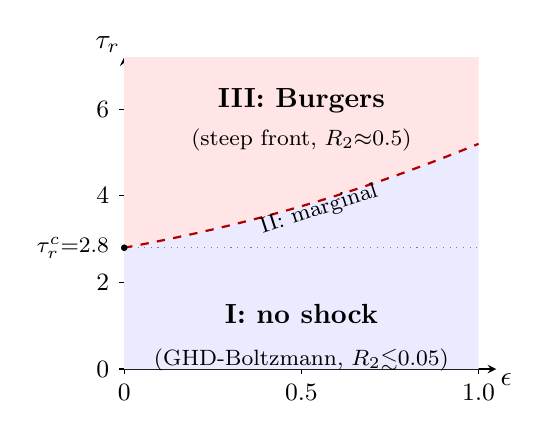
\begin{tikzpicture}[x=4.5cm, y=2.2cm]
  \draw[->,>=stealth] (0,0) -- (1.05,0)
        node[below right=-2pt]{$\epsilon$};
  \draw[->,>=stealth] (0,0) -- (0,1.8)
        node[above left=-2pt]{$\tau_r$};
  \foreach \x/\xl in {0/0, 0.5/0.5, 1.0/1.0}
    \draw (\x,0) -- (\x,-0.03) node[below]{\small$\xl$};
  \foreach \y/\yl in {0/0, 0.5/2, 1.0/4, 1.5/6}
    \draw (0,\y) -- (-0.015,\y) node[left]{\small$\yl$};

  \fill[blue!8] (0,0) -- (0,0.7) .. controls (0.4,0.85) and
        (0.7,1.05) .. (1.0,1.30) -- (1.0,0) -- cycle;
  \fill[red!10] (0,0.7) .. controls (0.4,0.85) and
        (0.7,1.05) .. (1.0,1.30) -- (1.0,1.8) -- (0,1.8) -- cycle;
  \draw[thick,dashed,red!70!black] (0,0.7) .. controls
        (0.4,0.85) and (0.7,1.05) .. (1.0,1.30);
  \draw[dotted,gray] (0,0.7) -- (1.0,0.7);
  \fill[black] (0,0.7) circle (1.2pt)
        node[left,xshift=-2pt]
        {\footnotesize$\tau_r^c{=}2.8$};
  \node at (0.5,0.32) {\textbf{I: no shock}};
  \node[font=\footnotesize] at (0.5,0.05)
        {(GHD-Boltzmann, $R_2{\lesssim}0.05$)};
  \node at (0.5,1.55) {\textbf{III: Burgers}};
  \node[font=\footnotesize] at (0.5,1.32)
        {(steep front, $R_2{\approx}0.5$)};
  \node[font=\footnotesize,rotate=18] at (0.55,0.92)
        {II: marginal};
\end{tikzpicture}
\caption{Qualitative $(\epsilon,\tau_r)$ phase diagram for
shock onset in the mass-disordered hard-rod gas with
inelasticity $\epsilon$ and reaction-time delay $\tau_r$,
at the parameters of Ref.~\cite{PaperIII} ($U_0=0.5$,
$m_{\max}=5$, step IC). The dashed curve is the qualitative threshold
$\tau_r^c(\epsilon)$ from
Eqs.~\eqref{eq:tcoh_eps}--\eqref{eq:tcoh_tau}, with
elastic-limit value $\tau_r^c(0)\approx 2.8$
(Eq.~\eqref{eq:tauc}) and leading-order slope
$d\tau_r^c/d\epsilon|_{0}\approx 0.25$
(Eq.~\eqref{eq:slope}); the visual slope of the cartoon is
exaggerated for clarity. Region~I is the no-shock GHD--Boltzmann
regime of Refs.~\cite{PaperIII,PaperIV,PaperV}; region~III
is the developed-Burgers regime characteristic of traffic
jam waves~\cite{Sugiyama2008,Bando1995}. The numerical
sweep of Sec.~\ref{sec:numerical} traces the
$\epsilon=0$ axis to locate $\tau_r^c(0)$ quantitatively.}
\label{fig:phase}
\end{figure}

\section{Numerical test of the shock-onset threshold}
\label{sec:numerical}

A direct numerical test of Eq.~\eqref{eq:tauc} requires an
event-driven hard-rod integrator augmented with a
reaction-time delay; we summarise here the planned protocol
and the quantitative signature to be measured.

\paragraph*{Protocol.} Event-driven mass-disordered hard-rod
dynamics at the parameters of Ref.~\cite{PaperIII}
($L=12.57$, $\sigma=0.00314$, $\rho^{\rm tot}=31.82$,
$\eta=0.1$, $m_{\max}=5$, $T=1$), with step-velocity IC
$\bar u(s,0)=U_0\,\mathrm{sgn}[\cos k_1 s]$ at $U_0=0.5$.
The delay channel is implemented as a \emph{contact-freeze}
modification of the elastic collision rule: at the contact
event $t_c$, both rods instantaneously adopt their
common arc-length velocity
$v_{\rm min}=\min(v_i, v_j)$ and remain in contact at this
shared velocity for the duration $\tau_r$; at
$t_c+\tau_r$ the full elastic velocity exchange
Eq.~(4) of Ref.~\cite{PaperIV} is applied. This protocol
preserves the cyclic-order invariant of the hard-rod
algorithm (rods cannot pass through one another during the
freeze) and reduces to the standard event-driven dynamics
in the $\tau_r\to 0$ limit. It is the natural hard-rod
analogue of the OVM reaction-time delay~\cite{Bando1995}:
the driver-like response (full velocity adjustment) is
delayed by $\tau_r$, but the immediate collision constraint
(no overlap) is enforced instantaneously. The inelastic
channel is fixed at $\epsilon=0$ to isolate the delay-only
shock onset.

\paragraph*{Sweep and observables.} The protocol sweeps
$\tau_r\in\{0, 1.0, 2.0, 2.5, 3.0, 3.5, 4.0\}$, bracketing
the analytical threshold $\tau_r^c\approx 2.8$ of
Eq.~\eqref{eq:tauc}. The principal observable is the
density-mode amplitude ratio
$R_n(t)\equiv|\hat\rho_n(t)|/|\hat\rho_1(t)|$ at the first
local maximum of $|\hat\rho_1|$, evaluated for $n=2,\ldots,7$.
The diagnostic signature of shock onset is the
\emph{appearance of even modes} of comparable magnitude to
the odd modes. In the linear regime the step IC excites only
odd-$n$ wavenumbers Fourier components ($\hat\rho_n=0$ for
even $n$ at $t=0$) and the GHD--Boltzmann linearised
dynamics preserves this parity to leading order, giving
the $R_n\sim 1/n$ cascade restricted to odd $n$
(Ref.~\cite{PaperIV} and Ref.~\cite{PaperV} Sec.~VIII for
the explicit even-mode noise floor at $U_0=0.05$). The
formation of a Burgers shock breaks this parity: at the
shock face, the locally steep gradient mixes even and odd
modes through the quadratic $u\,\partial_x u$ nonlinearity,
yielding even-mode amplitudes that scale as
$|\hat\rho_{2m}|/|\hat\rho_1|\sim (U_0/c_s)^m$ for the
$m$-th even harmonic. A clean shock-onset diagnostic is
therefore the \emph{relative even-mode amplitude}
$R_2\equiv|\hat\rho_2|/|\hat\rho_1|$ at the first
maximum of $|\hat\rho_1|$, in which the large fundamental
$|\hat\rho_1|$ in the denominator suppresses statistical
noise relative to denominators built from higher harmonics.
In the GHD--Boltzmann no-shock regime
Ref.~\cite{PaperV} (Table~VI) reports $R_2\approx 0.043$ at
$U_0=0.5$, i.e.\ even modes suppressed by more than an order
of magnitude relative to the fundamental. In the developed
Burgers regime the inviscid-Burgers cascade
$|\hat\rho_n|/|\hat\rho_1|\to 1/n$ (in suitable
sawtooth-coordinate frames) gives $R_2\to 1/2$, a
factor of ten above the no-shock floor.

\paragraph*{Expected result.}
For $\tau_r<\tau_r^c$: phase mixing pre-empts shock
formation, $R_2$ remains at the no-shock floor
$R_2\lesssim 0.05$ (Ref.~\cite{PaperV}).
For $\tau_r\approx\tau_r^c$: $R_2$ rises as the quadratic
mode-mixing channel opens but the cascade is incomplete.
For $\tau_r>\tau_r^c$: $R_2\to 0.5$, signalling the
developed Burgers cascade.

The quantitative match between the threshold extracted
from the $R_2(\tau_r)$ data and the analytical prediction
Eq.~\eqref{eq:tauc} is the falsifiable claim of the
present construction. The implementation and a complete
report of the sweep are deferred to a companion data
release.

\section{Discussion}\label{sec:discussion}

\subsection{Position relative to existing literature}

\emph{Kinetic theory of traffic.} The microscopic-to-mesoscopic
projection developed here parallels the
Prigogine--Herman--Paveri-Fontana tradition~\cite{
PrigogineHerman1971} and its modern Klar--Wegener and
Helbing-type extensions~\cite{Klar1996,Helbing2001}. The
present work differs in starting from a controlled
microscopic substrate (the integrable hard-rod gas of
Refs.~\cite{PaperI,PaperII,PaperIII,PaperIV,PaperV}) rather
than from a phenomenological Boltzmann-type ansatz on the
desired-velocity distribution.

\emph{Reductive-perturbation derivations of Burgers from
car-following.} Komatsu and Sasa~\cite{Komatsu1995},
Nagatani~\cite{Nagatani1999}, and others have derived the
Burgers, KdV, and mKdV equations in different stability
regions of the OVM by reductive-perturbation methods. The
present work derives the \emph{stochastic} Burgers as the
mesoscopic object and identifies the
$(\epsilon, \tau_r, D)$-parametric origin of the deterministic
limit, distinguishing the noise-driven and noise-free regimes.

\emph{Inelastic GHD-Boltzmann.} The
collision integral $\mathcal{C}_{\rm coll}^{(\epsilon)}$ in
Eq.~\eqref{eq:fp} is the inelastic extension of the
GHD--Boltzmann kernel introduced in Ref.~\cite{PaperIV}.
Recent work on weak integrability breaking in GHD
\cite{DurninDoyon2021,WeakBreaking2023} treats elastic
energy-conserving perturbations; the inelastic channel
considered here is structurally distinct.

\subsection{Implications and open work}

The stochastic Burgers equation Eq.~\eqref{eq:stoch_burgers}
identifies the natural mesoscopic object connecting the
integrable hard-rod baseline with the shock-dominated
continuum. The KPZ-class long-wavelength fluctuations
encoded in $f(x,v,t)$ are accessible both numerically (via
event-driven simulation of
Eqs.~\eqref{eq:micro1}--\eqref{eq:micro2} with the
contact-freeze collision rule of Sec.~\ref{sec:numerical})
and analytically via the well-developed KPZ machinery
\cite{Hairer2013,QuastelSpohn2015}.
The principal open computational task is the direct
numerical determination of the threshold
$\tau_r^c(\epsilon, D)$ from the sweep of
Sec.~\ref{sec:numerical}, and its comparison against the
analytical prediction Eq.~\eqref{eq:tauc}.

For vehicular-traffic applications, the result implies that
coherent jam waves with sharp upstream fronts emerge only
when at least one of the three channels --- inelasticity,
reaction-time delay, or external driver noise --- is
sufficiently strong, and the delay channel is the dominant
shock-promoting ingredient (Sec.~\ref{sec:macro}). An
elastic, instantaneous, deterministic car-following model
cannot reproduce the empirical phenomenology of jam-wave
formation documented in Ref.~\cite{Sugiyama2008}.

\begin{acknowledgments}
This work was supported by Tecnol\'ogico de Monterrey.
\end{acknowledgments}

\appendix

\section{Inelastic collision and delay-memory kernels}
\label{app:kernels}

\subsection*{A.1 Inelastic two-body collision rule}

For a pair $(i,j)$ of particles of masses $(m_i, m_j)$ in 1D
with restitution coefficient $r=1-\epsilon\in[0,1]$, the
post-collision velocities are
\begin{align}
v_i' &= \frac{m_i - r\,m_j}{m_i+m_j}\,v_i
       + \frac{(1+r)\,m_j}{m_i+m_j}\,v_j, \\
v_j' &= \frac{(1+r)\,m_i}{m_i+m_j}\,v_i
       + \frac{m_j - r\,m_i}{m_i+m_j}\,v_j.
\label{eq:inel_coll}
\end{align}
The kinetic energy dissipated per collision is
\begin{equation}
\Delta E_{\rm coll} = \frac{1}{2}\,
\frac{m_i m_j}{m_i+m_j}\,(1-r^2)\,(v_i-v_j)^2
= \mu\,\epsilon(2-\epsilon)\,\tfrac12(v_i-v_j)^2,
\label{eq:dE}
\end{equation}
with reduced mass $\mu = m_i m_j/(m_i+m_j)$. The elastic
limit $r=1$ (i.e.\ $\epsilon=0$) recovers $\Delta E=0$ and the
collision rule of Ref.~\cite{PaperIV}; the fully inelastic
limit $r=0$ gives $\Delta E = \tfrac12\mu(v_i-v_j)^2$
(complete loss of relative kinetic energy, contact stickiness).
The collision kernel entering $\mathcal{C}_{\rm coll}^{(\epsilon)}$
in Eq.~\eqref{eq:fp} is constructed from
Eq.~\eqref{eq:inel_coll} in the standard Boltzmann form;
note that for $\epsilon>0$ the Jacobian of
$(v_i,v_j)\to(v_i',v_j')$ is $r=1-\epsilon$ (not unity), so
\begin{multline}
\mathcal{C}_{\rm coll}^{(\epsilon),\alpha}[f_L,f_H]
= \sigma\!\int dv'\,|v-v'|\\
\times\left[\frac{1}{r^2}\,f_\alpha(v_*)\,f_\beta(v'_*)
            - f_\alpha(v)\,f_\beta(v')\right],
\label{eq:Cinel}
\end{multline}
with $\beta\neq\alpha$ as in Sec.~II of Ref.~\cite{PaperIV},
with $(v_*,v'_*)$ the pre-collision pair that yields $(v,v')$
after Eq.~\eqref{eq:inel_coll}. The $1/r^2$ factor is the
standard Jacobian correction for inelastic kernels
\cite{BrilliantovPoschel}. The discrete-velocity implementation
of Eq.~\eqref{eq:Cinel} for $\epsilon>0$ requires the
$3$-point Lagrange Bobylev--Palczewski--Schneider interpolation
developed in Ref.~\cite{PaperV}, Sec.~III. With $r\neq 1$ the
post-collision velocities $v_i', v_j'$ are generically off-grid;
the bilinear $2$-point scheme suffices in the elastic case but
introduces an $O(\Delta v^2)$ discretisation error on top of
the physical $O(\epsilon)$ energy dissipation, contaminating
the inelasticity-induced loss with grid noise. The $3$-point
Lagrange scheme preserves \emph{mass} and \emph{momentum} to
machine precision for any $r\in[0,1]$ (these are the
collision invariants for elastic and inelastic
binary kernels alike), while the physical kinetic-energy
loss Eq.~\eqref{eq:dE} is reproduced cleanly without
grid-noise contamination. The thermal energy is exactly
conserved only for $r=1$; for $r<1$ the kinetic energy
decreases monotonically at the discrete rate set by
Eq.~\eqref{eq:dE}.

\subsection*{A.2 Delay memory kernel}

The reaction-time delay $\tau_r$ in
Eq.~\eqref{eq:micro2} replaces the instantaneous response
$F[v_j(t)]$ with $F[v_j(t-\tau_r)]$. Taylor-expanding for
$\tau_r$ smaller than the dynamical correlation time,
$v_j(t-\tau_r) = v_j(t) - \tau_r\,\dot v_j(t)
+ O(\tau_r^2)$, and substituting $\dot v_j$ via
Eq.~\eqref{eq:micro2} itself yields a closed-form
modification of the streaming and collision terms. At the
Fokker--Planck level this generates a memory operator
\begin{equation}
\mathcal{C}_{\rm delay}^{(\tau_r)}[f]
= -\tau_r\,\partial_v\!\left[\bar F(x,v,t)\,f\right]
+ O(\tau_r^2),
\label{eq:Cdel}
\end{equation}
with $\bar F$ the mean-field drift induced by the
delay-coupled neighbour state. The form Eq.~\eqref{eq:Cdel} is
a renormalisation of the streaming term; at leading order in
$\tau_r$ it contributes to the effective viscosity
$\nu_{\rm eff}$ in Eq.~\eqref{eq:stoch_burgers} (a similar
mechanism produces the OVM-derived Burgers viscosity of
Komatsu and Sasa~\cite{Komatsu1995}).

\section{Effective transport coefficients}
\label{app:prefactors}

The effective viscosity $\nu_{\rm eff}(\epsilon,\tau_r)$ and
noise intensity $D_{\rm eff}(\epsilon,D)$ in
Eq.~\eqref{eq:stoch_burgers} are obtained by Chapman--Enskog
expansion of the Fokker--Planck equation~\eqref{eq:fp} about
the binary-Maxwell local equilibrium of Ref.~\cite{PaperIV}.

\subsection*{B.1 Elastic baseline $\nu_0$}

In the strict $\epsilon=\tau_r=0$ limit, the
one-dimensional elastic hard-rod gas has no Newtonian
viscosity: the off-diagonal stress vanishes identically
and the bulk viscosity is zero because pressure and energy
density are thermodynamically dependent
(Ref.~\cite{PaperV}, Sec.~V). The only finite Chapman--Enskog
transport coefficients are the binary interdiffusion
$D_{LH}\approx 4$ and the thermal conductivity
$\lambda_T(m_{\max})$ (Ref.~\cite{PaperV}, Sec.~V). The
``effective Burgers viscosity'' $\nu_0$ that enters
Eq.~\eqref{eq:stoch_burgers} is therefore not a microscopic
shear viscosity but the apparent diffusion of the
mean-velocity field induced by the kinetic phase-mixing of
the underlying species-resolved distribution; numerically,
the resulting damping rate of the linearised sound mode at
$k_1=2\pi/L$ is set by the inter-species collision rate
$\tau_{\rm break}^{-1}\approx 0.1$
(Ref.~\cite{PaperV}, Sec.~VII), giving
$\nu_0^{\rm eff}\sim\tau_{\rm break}^{-1}/k_1^2\approx 0.4$
as the effective viscosity entering
Eq.~\eqref{eq:stoch_burgers} at $\epsilon=\tau_r=0$.

\subsection*{B.2 Inelastic contribution $\nu_\epsilon$}

The dissipated kinetic energy per unit time per unit volume
from Eq.~\eqref{eq:dE} is $\dot E_{\rm diss} = \rho_0^2
\sigma\,\bar v\,\mu\,\epsilon(2-\epsilon)\,\langle(v-v')^2\rangle/2$;
identifying this with the viscous dissipation rate
$\eta(\partial_x u)^2$ at characteristic gradient $u_0 k$
gives the leading-order contribution
\begin{equation}
\nu_\epsilon = \frac{2 \mu\,\epsilon\,\sigma\,\bar v}{\bar m}
\;+\; O(\epsilon^2),
\label{eq:nu_eps}
\end{equation}
which for the binary mixture at $\epsilon\sim 0.1$ gives
$\nu_\epsilon \approx 0.06$, comparable to $\nu_0$ — a small
amount of inelasticity already doubles the effective
viscosity.

\subsection*{B.3 Delay contribution $\nu_\tau$}

The Taylor expansion of $\bar F$ in Eq.~\eqref{eq:Cdel}
produces an effective gradient-dependent drift, which at the
hydrodynamic level adds
\begin{equation}
\nu_\tau = c_s^2\,\tau_r\;+\;O(\tau_r^2),
\label{eq:nu_tau}
\end{equation}
in close analogy to the OVM kinetic
derivation~\cite{Komatsu1995}. For $\tau_r\sim 0.1$ and
$c_s\sim 1$, this gives $\nu_\tau\approx 0.1$.

\subsection*{B.4 Noise enhancement $D_\epsilon$}

A steady-state energy-balance argument relates the
inelastic dissipation rate to the noise required to
maintain stationarity. The fluctuation--dissipation
theorem in its equilibrium form does not apply to the
inelastic dynamics~\cite{BrilliantovPoschel}, and the
balance below should be read as the leading-order
relation between the Langevin noise power injected by
$\xi_i(t)$ and the inelastic energy loss rate, valid in
the weakly-inelastic, weakly-driven regime where
non-equilibrium corrections are subleading. Imposing this
balance gives
\begin{equation}
D_\epsilon \;\sim\; \nu_\epsilon\,k_BT/\bar m,
\end{equation}
so that $D_{\rm eff} = D + D_\epsilon$ grows approximately
linearly with $\epsilon$ at small $\epsilon$. In the
noise-driven limit $D\gg D_\epsilon$, the stochastic
Burgers equation Eq.~\eqref{eq:stoch_burgers} is in the
standard KPZ regime~\cite{KPZ1986}; in the
dissipation-dominated limit $D_\epsilon\gg D$, the
effective noise inherits the collisional correlation time
$\tau_{\rm break}$ as discussed in
Sec.~\ref{sec:meso}.

\begin{thebibliography}{99}

\bibitem{PaperI}
H.~Medel,
in preparation (2026).

\bibitem{PaperII}
H.~Medel,
in preparation (2026).

\bibitem{PaperIII}
H.~Medel,
in preparation (2026).

\bibitem{PaperIV}
H.~Medel,
in preparation (2026).

\bibitem{PaperV}
H.~Medel,
in preparation (2026).

\bibitem{HubnerDoyon2024}
F.~H\"ubner, B.~Doyon,
arXiv:2406.18322 (2024),
\url{https://arxiv.org/abs/2406.18322}.

\bibitem{Sugiyama2008}
Y.~Sugiyama, M.~Fukui, M.~Kikuchi, K.~Hasebe, A.~Nakayama,
K.~Nishinari, S.~Tadaki, S.~Yukawa,
New J.~Phys.\ \textbf{10}, 033001 (2008),
doi:10.1088/1367-2630/10/3/033001.

\bibitem{Lighthill1955}
M.~J.~Lighthill, G.~B.~Whitham,
Proc.~Roy.~Soc.~A \textbf{229}, 317 (1955),
doi:10.1098/rspa.1955.0089.

\bibitem{Bando1995}
M.~Bando, K.~Hasebe, A.~Nakayama, A.~Shibata, Y.~Sugiyama,
Phys.~Rev.~E \textbf{51}, 1035 (1995),
doi:10.1103/PhysRevE.51.1035.

\bibitem{Komatsu1995}
T.~S.~Komatsu, S.-i.~Sasa,
Phys.~Rev.~E \textbf{52}, 5574 (1995),
doi:10.1103/PhysRevE.52.5574.

\bibitem{Komatsu2003}
T.~Komatsu, T.~Nagatani,
Physica~A \textbf{332}, 449 (2003).

\bibitem{Treiber2000}
M.~Treiber, A.~Hennecke, D.~Helbing,
Phys.~Rev.~E \textbf{62}, 1805 (2000),
doi:10.1103/PhysRevE.62.1805.

\bibitem{BrilliantovPoschel}
N.~V.~Brilliantov, T.~P\"oschel,
\emph{Kinetic Theory of Granular Gases},
Oxford University Press (2004).

\bibitem{KPZ1986}
M.~Kardar, G.~Parisi, Y.-C.~Zhang,
Phys.~Rev.~Lett.\ \textbf{56}, 889 (1986),
doi:10.1103/PhysRevLett.56.889.

\bibitem{Hairer2013}
M.~Hairer,
Ann.~Math.\ \textbf{178}, 559 (2013).

\bibitem{QuastelSpohn2015}
J.~Quastel, H.~Spohn,
J.~Stat.~Phys.\ \textbf{160}, 965 (2015).

\bibitem{PrigogineHerman1971}
I.~Prigogine, R.~Herman,
\emph{Kinetic Theory of Vehicular Traffic},
Elsevier (1971).

\bibitem{Klar1996}
A.~Klar, R.~Wegener,
SIAM J.~Appl.~Math.\ \textbf{59}, 983 (1999).

\bibitem{Helbing2001}
D.~Helbing,
Rev.~Mod.~Phys.\ \textbf{73}, 1067 (2001),
doi:10.1103/RevModPhys.73.1067.

\bibitem{Nagatani1999}
T.~Nagatani,
Physica~A \textbf{264}, 581 (1999).

\bibitem{DurninDoyon2021}
J.~Durnin, M.~J.~Bhaseen, B.~Doyon,
arXiv:2103.11997 (2021),
\url{https://arxiv.org/abs/2103.11997}.

\bibitem{WeakBreaking2023}
A.~Bastianello, A.~De~Luca, B.~Doyon, J.~De~Nardis,
arXiv:2302.12804 (2023),
\url{https://arxiv.org/abs/2302.12804}.

\end{thebibliography}

\end{document}
